%!TeX ts-program = xelatex
%!TeX encoding = utf-8 Unicode
\documentclass[ieeetran]{article}
\usepackage{amsmath, amssymb}
\usepackage{graphicx}

\title{Software Engineering for Business Applications Lecture Notes}
\author{Efe Kamasoglu}

\begin{document}

\maketitle

\pagebreak

\section{IT Support for Business Applications} % (fold)
\label{sec:iT_support_for_business_applications}

\subsection{Classification of Business Applications} % (fold)
\label{sub:classification_of_business_applications}

\begin{itemize}
  \item \textbf{Definition "Business Application":}
	  \begin{itemize}
	    \item \underline{in narrower sense:} totality of all programs, i.e.\ \textbf{application software}, and associated \textbf{data} for a concrete business use case
	    \item \underline{in broader sense:} additionally \textbf{hardware}, \textbf{system software} and necessary \textbf{communication} facilities required for the use of application software
	  \end{itemize}
\item \textbf{Two roles of Business Applications:}
	\begin{itemize}
	  \item \textbf{supporting}, \textbf{improving} or \textbf{automating} existing operational processes in bookeeping, accounting, etc.\ (size, speed, correctness...)
	\item \textbf{enabling} new products and services (e.g.\ online shopping and banking)
	\end{itemize}
\item \textbf{Classification of Business Applications by Business Purpose:}
	\begin{figure}[h!]
	  \centering
	  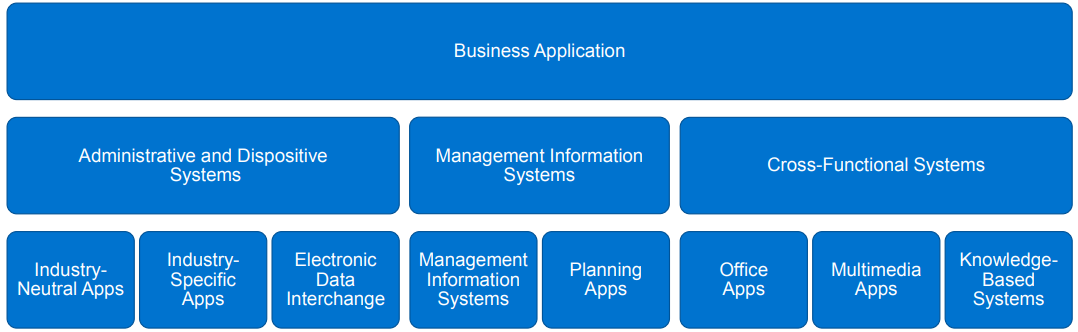
\includegraphics[width=0.5\linewidth]{classofba.png}
	  \label{fig:classofba_png}
	\end{figure}

\textit{\underline{Examples of}}

\begin{itemize}
  \item \textbf{administrative systems:} financial accounting, payroll accounting, administration of stocks
\item \textbf{disposition systems:}\ calculation and cost accounting, material procurement, field service control
\item \textbf{management information systems (MIS):} use of internal company data, use of external data, combination of multiple data sources in a flexible form
\item \textbf{planning systems:}\ planning of individual functional areas, integrated planning of several functional areas, corporate planning

\end{itemize}
\item \textbf{Cross-Cutting Applications:}
	\begin{itemize}
	  \item independent of compant hierarchy and fuctional domains
	\item used either directly via user interface or programmatically via administration and disposition systems
	\item \textit{Examples:} office suites, groupware, workflow management systems
	\end{itemize}

\item \textbf{Enterprise Resource Planning (ERP):} \textbf{ERP system} is an integrated business application (suite, collection of programs), which supports all essential functions of administration, disposition and management with a \underline{common interface and a shared and integrated data management}.
	\begin{itemize}
	  \item consists of platform and function-oriented application components that exchange info and events
          \item is realized as (customizable) standard software
	\item \textit{Examples:} external accounting, controlling, procurement
	\item Today's ERP systems support an \textbf{extended value chain}\footnote{\textbf{Value chain} is a business model that describes the full range of activities needed to create a product or service.}.
	\end{itemize}
\end{itemize}

\subsection{Standard and Custom Software} % (fold)
\label{sub:standard_and_custom_software}

\begin{itemize}
  \item \textbf{Standard Software vs. Custom Software:}
	  \begin{itemize}
	    \item \textbf{Standard software} \textit{(e.g.\ SAP)}
		    \begin{itemize}
		      \item developed for specific \textbf{market}
		\item distributed by a software house
			\item can be used by \textbf{several companies}
			\item implements "standard business processes" at its core
			\item maintained by \textbf{manufacturer}, adapted to changes
			\item must or can be \textbf{customized} to company (e.g.\ authorizations and roles, currencies) 
		    \end{itemize}
	\item \textbf{Custom software}
		\begin{itemize}
		  \item specifically developed for \textbf{one company}
	\item tailored to specific business processes/requirements
		\item result of a project for a known client
			\item \textbf{individually} maintained and adapted to changes
		\end{itemize}
	  \end{itemize}
\pagebreak
\item \textbf{Adaptation Techniques for Standard Business Software:}
	\begin{itemize}
		\item Adaptation of operational standard software can be divided into \textbf{Configuration}, \textbf{Extension} and \textbf{Coupling} (= \textbf{Customizing}).
               \begin{figure}[h!]
                 \centering
                 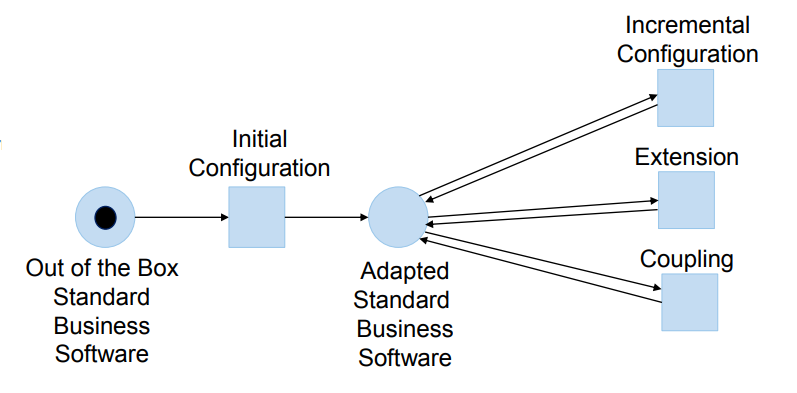
\includegraphics[width=0.5\linewidth]{adaptationsbs.png}
                 \label{fig:adaptationsbs_png}
               \end{figure} 

	       \item \textbf{Configuration} describes functionalities and techniques
		       \begin{itemize}
		         \item that are obligatory on first deployment
				 \item that allow to define predefined settings
			\item that lead to an individual variation of standard software
		       \end{itemize}

	\item \textbf{Extension} describes functionalities and techniques
		\begin{itemize}
		  \item that are optional for productive use
			  \item that allow to map requirements not foreseen by manufacturer
				  \item implemented by manufacturer to expand the range of services
		\end{itemize}

		\item \textbf{Coupling} refers to functionalities and techniques
			\begin{itemize}
			  \item to connect external systems of other manufacturers
				  \item to connect external systems of the same type
				\item that are predefined in the form of data file formats, APIs, or communication protocols
			\end{itemize}


		\item \textit{Example:} mapping the structure of a company to SAP applications via organizational units (can be assigned to single or multiple apps)
	\end{itemize}

	\item \textbf{Configuration: Challenges}
		\begin{itemize}
		  \item A \textbf{standard software} must
			  \begin{itemize}
			    \item provide all relevant configuration options
			\item support a wide range of different corporate structures and processes
			\item check dependencies between these many variants
			\item provide appropriate documentation about the effects of individual configurations

			  \end{itemize}
		  \item \textbf{Consequences:} 
				  \begin{itemize}
				    \item need for experts who are familier with configuration options of each release and componant
					   \item scarcity of such experts
						   \item expensive training
							   \item expensive consultancy services
				  \end{itemize}
		\end{itemize}

\item \textbf{Examples for Extensions:}
	\begin{itemize}
	  \item automation of \textbf{multi-step business workflows}
	\item integration of company-specific calculations/rules/checks
	\item connecting customers
	\end{itemize}
\item \textbf{Coupling Options:}
	\begin{itemize}
	  \item different coupling options depending on the scenario
	\item programming language used for coupling
	\item available mechanisms to couple
	\end{itemize}

\item \textbf{Multi Tenancy:} Software multitenancy is a software architecture in which a single instance of software runs on a server and serves multiple tenants (e.g.\ companies).
	\begin{itemize}
	  \item sevearal companies can be represented in one system
	\item distinction between tenant-dependent and -independent data
	\item supporting tenant-dependent authorization (e.g.\ A may only perform transactions in client 002)
         \item individual adaptations of tenants (e.g.\ currency, couplings)
	\end{itemize}

\item \textbf{Multilingualism:}

	\begin{itemize}
	\item \textbf{Multilingualism of a business information system} makes it possible to
		\begin{itemize}
		  \item store and display texts in different languages in the system
		\item assing graphics and symbols specific to different languages 
		\end{itemize}
	
\item Multilingualism requires
	\begin{itemize}

\item that one system can process all relevant character sets at once
	\item storage and recognition of words, numbers etc.
	\item that a system can assign users to languages or user can choose their own
	\item that texts (graphics, symbols) can be assigned to a language
	\end{itemize}
	\end{itemize}
\item \textbf{Localization (l10n):} Adaptation of a software product to meet the language, culture, and other requirements of each locale (e.g.\ adaptation of graphics, currencies, date and time)
\item \textbf{Internationalization (i18n):}\ Process of preparing a software-based product for localization (to support global markets)
\end{itemize}

\subsection{Characteristics of Business Applications} % (fold)
\label{sub:characteristics_of_business_applications}
\begin{itemize}
  \item \textbf{Multiple Stakeholders and changing requirements:}
	  \begin{itemize}
	    \item \textbf{Requirements Elicitation and Requirements Management}
		    \begin{itemize}
		      \item many stakeholders, different views and concerns
		\item Waterfall: upfront requirements document and/or technical specification => Req. Documentation
		\item Issue: changing requirements once IT support is implemented
		\item Agile: incremental and iterative => Agile Req. Engineering
			\item typically, very large number of requirements
			\item need for formalization and early consistency checking => Conceptual Modeling
				\item need for cost and time prediction => Software Estimation

		    \end{itemize}

	\item \textbf{Programming Challenges}
		\begin{itemize}
		  \item design, implement and test changes in an existing complex system => Change Mgmt.
	\item deliver incremental changes without invalidating existing data => Release Mgmt.
		\item parallel development at manufacturer and at customer site => Version Mgmt.

		\item automated and quality-controlled assembly of application software => Build Mgmt.
		\end{itemize}
	  \end{itemize}

\item \textbf{Persistent Data and Concurrent Data Modification:}
	\begin{itemize}
	  \item \textbf{Data consistency} is a must:
		  \begin{itemize}
		    \item many users perform \textbf{transactions} simultaneously on central databases
		\item data must not be lost even in case of system failures.
		  \end{itemize}
		  \item \textbf{Programming challenges:}
			  \begin{itemize}
			    \item database is managed by an independent application, on a different server / hardware
			\item object orientation is not supported by common data bases
				\item database concepts must be transferred to the application logic (transactions, rights, primary keys)
			  \end{itemize}
	\end{itemize}

\item \textbf{Distributed Actors and Data Repositories:}
	\begin{itemize}
	  \item \textbf{Many users access central data concurrently:}
		  \begin{itemize}
		    \item users need data in different locations at different times
			    \item Client-Server architecture => Layered Architectures
		\item web clients => REST protocol
		  \end{itemize}

	\item \textbf{Programming challenges:}
		\begin{itemize}
		  \item software components must be able to found in network => Naming services
		  \item communication always via a network => Serialization\footnote{\textbf{Serialization} is the process of translating a data structure into a format that can be stored or transmitted and reconstructed later.} \& failed execution
			  \item authentication and authorization => Security
		\item concurrent accesses => Transactions
		\end{itemize}
	\end{itemize}

\item \textbf{Integeration of Data and Application from (Semi-)Autonomous Sources:}
	\begin{itemize}
	  \item \textbf{Separation of applications and data repositories:}
		  \begin{itemize}
		    \item multiple apps work on independent or shared data resources
			    \item multiple apps communicate with each other => RPC, Message Passing
			\item business processes involve multiple apps => Workflow Mgmt. Systems
			\item application landscapes with lots of interacting applications => Enterprise Architecture Mgmt.
		  \end{itemize}

		  \item \textbf{Programming challenges:}
			  \begin{itemize}
				  \item integration of multiple languages and databases
				\item loose coupling through interfaces to avoid code change propagationi
				\item error recovery to avoid runtime failure propagation
			  \end{itemize}
	\end{itemize}

\item \textbf{Scalability:}
	\begin{itemize}
	  \item \textbf{Growing number of users and data volume}
		  \begin{itemize}
		    \item business apps are used by thousands of employees world-wide around the clock
		\item customers and business partners interact directly with business apps and expect real-time sub-second response times
		\item volatile load (e.g.\ online shop in christmas season vs.\ summer season)
		  \end{itemize}
		  \item \textbf{Programming challenges:}
			  \begin{itemize}
				  \item delayed execution of resource-intesive operations => Batch processing\footnote{\textbf{Batch processing} is when a computer processes a number of tasks that it has collected in a group. It is designed to be a completely automated process, without human intervention.}
				    \item dynamically increasing/decreasing number of users => Instance pools
					    \item single server cannot handle the load => Load balancing, Caching
		
			  \end{itemize}
	\end{itemize}
\end{itemize}

\section{Requirements Engineering} % (fold)
\label{sec:requirements_engineering}

\begin{itemize}

\item \textbf{Software requirements} express the needs and constraints placed on a software product.

  \item \textbf{Requirements engineering} is concerned with \textbf{elicitation}, \textbf{analysis}, \textbf{specification} and \textbf{validation} of software requirements as well as the management of requirements.

\item \textbf{Requirements Management} deals with the administration and maintenance of requirements documents, in particular:
	\begin{itemize}
	  \item change requirements (change management)
          \item trace and link requirements (requirements tracing)
	  \item verify requirements
	\end{itemize}


\end{itemize}

\subsection{Traditional Requirements Engineering} % (fold)
\label{sub:traditional_requirements_engineering}

\begin{itemize}
	\item \textbf{Objectives of Requirements Management:}
		\begin{itemize}
		  \item \textbf{Efficient} preparation of \textbf{high quality} requirements and system specifications,
			   \begin{itemize}
			     \item coordinated with all stakeholders (different objectives and interests)
			\item coordinated with all specifications and constraints
			\item evaluated according to profitability and feasibility 
			   \end{itemize}

		\item \textbf{Specification documents} are basis for:
			\begin{itemize}
			  \item contract negotiation and contractual agreements
		\item coordination between the stakeholders (customers, developers)
		\item design, realization, integration
			 \item software acceptance (test specification)
			\item future developments, projects
			\end{itemize}
		\end{itemize}
\item \textbf{Requirement Classification:} Distinction between \underline{functional and non-} \underline{functional requirements and constraints}:
	\begin{itemize}
		\item \textbf{Functional requirements} \ describe \underline{interactions} between the system and its environment independent of their realization.
		\item \textbf{Non-functional requirements} describe \underline{general properties} of the system.
\item \textbf{Restrictions (Constraints)} determine the \underline{solution space} for the realization.	
	\end{itemize}

\item \textbf{Stakeholder Management:} It includes
	\begin{itemize}
	  \item processes required to identify people that could impact or be impacted by the project
\item to analyze stakeholder expectations and their impact on the project
	\item to develop appropriate management strategies for effectively engaging stakeholders in project decisions and execution
	\end{itemize}

\item \textbf{Requirement Specification:}
	\begin{itemize}
	  \item technical result document of requirement identification phase
	\item \textbf{contains} \underline{stakeholder identification, functional and non-functional}\\ \underline{requirements, constraints, evaluation plan and metrics}
	\item list of all deliverables and services to be fulfilled by contractor within contract as defined by customer
	\item \textbf{what} is to expect from the solution (product)
	\item formulation of requirements should be as general as possible and as restrictive as necessary
	\item enables the contractor to develop optimal solutions
	\end{itemize}

\item \textbf{Requirements Validation:} \textbf{Validation}, \textbf{Consistency check} (no conflicts), \textbf{Completeness check}, \textbf{Reality check}, \textbf{Verifiability}

\item \textbf{Functional Specification:}
	\begin{itemize}
	\item defines the purpose of the system
	  \item solution proposal created by contractor based on the requirement specification provided by client
		  \item \textbf{contains} \underline{target determination, product usage, environment (e.g.}\\ \underline{hardware), functions, UI, global test cases} 
	\item system description or solution specification, which describes \textbf{how} the solutions is to be realized (concrete solution approaches)
	\item the \textbf{what} from \textbf{requirement specification} is detailed
	\end{itemize}
\end{itemize}

\subsection{Agile Requirements Engineering} % (fold)
\label{sub:agile_requirements_engineering}

\begin{itemize}
  \item \textbf{Requirements Engineering and Agile Software Development:}
\begin{itemize}
  \item \textbf{Agile software development} focuses more on \textbf{continuous collabration} (workshops, interviews etc.) with stakeholders instead of relying on \textbf{specification documents} (\textit{example: SCRUM})
	  \item \textbf{Traditional requirements engineering}
		  \begin{itemize}
		    \item focuses on customer collabration mainly at an \underline{early phase of the} \underline{project} (longer change cycles)
			   \item emphasizes a heavy-weight process with extensive, \textbf{static specification documents}
				   
		  \end{itemize}


\item \textbf{Agile requirements engineering}
	\begin{itemize}
		\item fosters communication with the customer during the \underline{whole development}\\ \underline{process} to \textbf{continuously update requirements}
		\item focuses less on extensive documentation, but specification documents \textbf{might be necessary} because of legal or contracting reasons etc.
		\item includes activities and artifacts that are similar to classical requirements engineering activities
	\end{itemize}
\end{itemize}

\item \textbf{Typical Requirement Artifacts in Agile Software Development:}
	\begin{itemize}
	  \item \textbf{user story}, \textbf{story card}, \textbf{use case}, \textbf{scenario}, \textbf{UML diagram}, \textbf{prototype}
	\end{itemize}

\item \textbf{User Stories:}
	\begin{itemize}
	  \item explanation of a software feature written from the perspective of the end user
		  \item most frequently used artifact in \textbf{agile software development}
		  \item mnemonic for writing good user stories: INVEST\footnote{independent, negotiable, valuable, estimable, small, testable}
	\end{itemize}

\item \textbf{Typical Requirements Engineering Challenges:}
	\begin{itemize}
	  \item different interest groups can raise \textbf{conflicting requirements}
	\item the people who \textbf{pay} for the system are rarely the ones who \textbf{use} it
	\item the organization and the technical environment may \textbf{change} after the system rollout
	\item requirements that change during implementation (Change Requests) can lead to additional costs -> project duration/milestones can be affected significantly
	\end{itemize}
\end{itemize}


\section{Conceptual Modeling with UML} % (fold)
\label{sec:conceptual_modeling_with_uML}

\begin{itemize}
\item \textbf{Conceptual Class Diagram vs.\ Implementation-Oriented Diagram:}
\begin{figure}[h!]
  \centering
  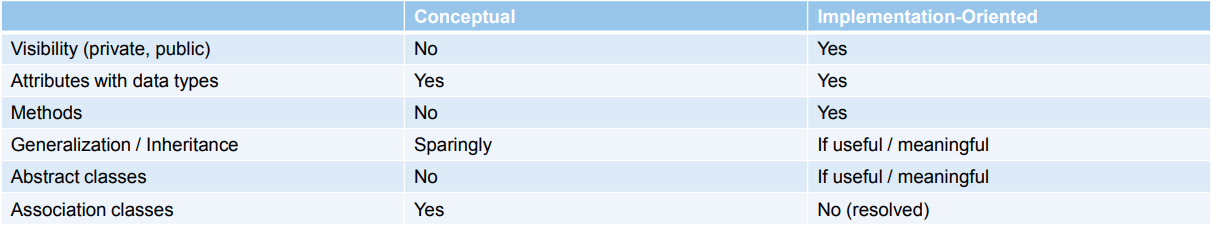
\includegraphics[width=1.0\linewidth]{umlcomparison.png}
  \label{fig:umlcomparison_png}
\end{figure}
\item \textbf{Associations between Classes:}

\pagebreak

\begin{itemize}
  \item \textbf{Multiplicity:}
	  \begin{figure}[h!]
	    \centering
	    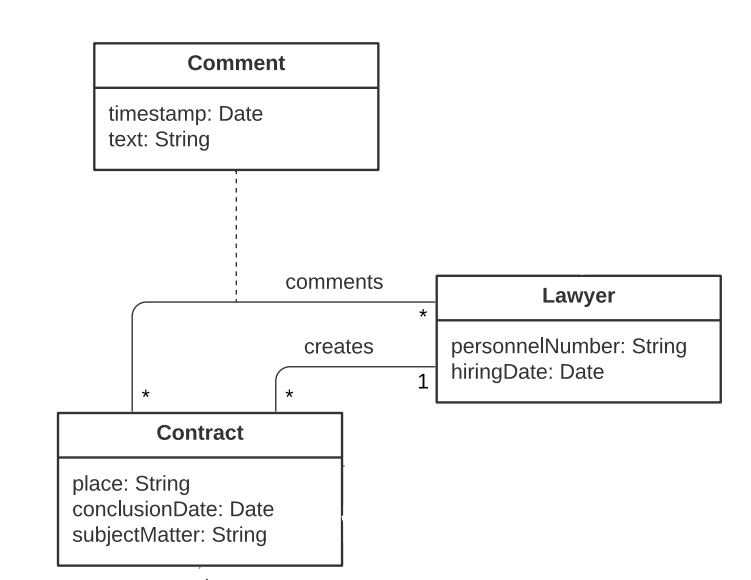
\includegraphics[width=0.5\linewidth]{umlmultiplicity.png}
	    \label{fig:umlmultiplicity_png}
	  \end{figure}
	  \\
	  \end{itemize}
	  \textit{
A Lawyer can \underline{create} \textbf{multiple} Contracts, whereas every Contract has a \textbf{single} Lawyer.
} -> \underline{creates} (action) on the side of Lawyer (actor)

\item \textbf{Aggregation:} implies a relationship where the child can exist independently of the parent (part of the parent)
\item \textbf{Composition:} implies a relationship where the child \underline{cannot exist} independent of the parent

\item  \textit{\underline{Example:}}
	\begin{figure}[h!]
	  \centering
	  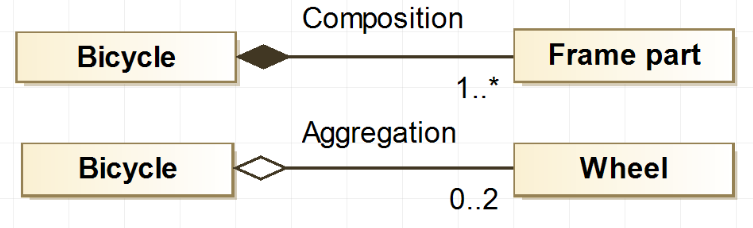
\includegraphics[width=0.4\linewidth]{compagg.png}
	  \label{fig:compagg_png}
	\end{figure}

\end{itemize}


\section{Software Estimation} % (fold)
\label{sec:software_estimation}

\subsection{Fundamentals of Estimation Methods} % (fold)
\label{sub:fundamentals_of_estimation_methods}
\begin{itemize}
  \item \textbf{Software Estimation:}
\begin{itemize}
  \item In principle, software estimation relies on \textbf{forecasting effort}, from which cost and duration are derived.
\item Regardless of the project and software methodology applied, every initiative requires the definition of a \textbf{budget} and a specific \textbf{time frame} necessary to deliver a final outcome.

\item These two are obtained during the \textbf{early stages} of the project lifecycle through the process of estimation.
\item \textbf{Estimation} aims to provide an \textbf{approximation} of the amount of recources required to complete project activities and produce a product or service in accordance to specified \textbf{functional} and \textbf{non-functional characteristics}.

\item \textbf{Software estimation conducted in early phases of the project lifecycle:}
	\begin{itemize}
	  \item necessary for contract negotiations
	\item predict expected efforts (and derived costs) for a software project before implementation
         \item best possible estimation given the available info
	\end{itemize}

\item \textbf{Agile estimation:}
	\begin{itemize}
	  \item estimation of individual requirements during project
	\item incremental allocation of developers in the most efficient manner
	\item cost estimates are made several times during development project with varying degrees of detail
	\end{itemize}
\end{itemize}
\item \textbf{Software Estimation: Cone of Uncertainty}
	\begin{itemize}
	  \item At the beginning of the project, not much is known about the product/project -> estimates underly high uncertainty
		  \item As the project progresses, more information is available -> decrease in uncertainty
	\end{itemize}
\item \textbf{Software Estimation: Costs}
	\begin{itemize}
	  \item \textbf{Cost categories:}
		  \begin{itemize}
		    \item \textbf{Development costs:} costs to produce a software product
			\item \textbf{Personnel costs:} major share of development costs for personnel
				\begin{itemize}
				  \item usually low costs for office materials etc.\ in relation to the personnel costs
				  \item proportionate allocation of CASE\footnote{Computer power-assisted software package Engineering} environment costs (including hardware and software) for product development
				\end{itemize}
		  \end{itemize}
	\end{itemize}
\end{itemize}

\subsection{Traditional Software Estimation} % (fold)
\label{sub:traditional_software_estimation}

\begin{itemize}
  \item \textbf{Sneed's Devil's Square:}
	  \begin{itemize}
	    \item Quantity
	\item Quality 
	\item Development duration
	\item Cost		
	  \end{itemize}
are mutually dependent.

\item \textbf{Quantity:}
	\begin{itemize}
		\item size of program code (example basis of assesment: LOC\footnote{Lines of Code})
		  \item functional and data scope
			  \item possible additional weighting with complexity
	\end{itemize}

\item \textbf{Quality:}
	\begin{itemize}
	  \item higher quality requirements => greater effort
	\item no \textbf{THE quality}, but different quality characteristics
	\end{itemize}

\item \textbf{Productivity:}
	\begin{itemize}
	  \item influenced by many different factors
	\item number of communication links grows \textbf{quadratically} with the team size
	\end{itemize}

\item \textbf{Development time:}
	\begin{itemize}
	  \item need more members to shorten development time
	\item more members => more communication effort
	\item higher communication => decrease in productivity
	\end{itemize}

\item \textbf{Methods for Effort Estimation:}
\begin{itemize}
  \item \textbf{Estimation Strategies:}
	  \begin{itemize}
	    \item \textbf{Top-Down:} estimation of the total project effort using mathematical algorithms based on the functional requirements
	\item \textbf{Bottom-Up:} expenses for each expense item are calculated separately and added to calculate the total project effort
	  \end{itemize}

\item \textbf{Comparison methods:}
	\begin{itemize}
	  \item estimation based on effort analysis of already accomplished similar developments
	\end{itemize}


\item \textbf{Algorithmic methods:}
	\begin{itemize}
	  \item effort calculated with algorithmic methods
	  \item based on statistical models or actual expenditure of already completed projects
	\end{itemize}

\item \textbf{Key figure methods:}
	\begin{itemize}
	  \item total cost of the software product determined by estimating the cost of individual units or project phases
	\end{itemize}

\item None of the listed basic methods alone is sufficient.
\item Depending on the point in time and knowledge of effort-relative data, one or the other method should be used.
\end{itemize}

\item \textbf{Concrete Procedures for Effort Estimation:}
	\begin{itemize}
	  \item \textbf{Goal:} Combine advantages of several effort estimation methods to deliver accurate results. (\textit{example: Function Point Method})
	\end{itemize}

\item \textbf{Function Point Method:} It is a combined relation and weighting method.
	\begin{enumerate}
	  \item \textbf{Categorization} of each product requirement (input, query, output, database, reference data)i
		  \begin{itemize}
		    \item \textbf{Input:} by the user
		\item \textbf{Output:} displaying query results, calculated data
		\item \textbf{Query:} performed on the \textbf{database} of the system, read and write
		\item \textbf{Reference data:} used to validate input, generate the output or construct the query (read-only)
		  \end{itemize}
\item \textbf{Classification} of each product requirement
	\begin{itemize}
	  \item \textbf{simple}
	  \item \textbf{medium} 
	  \item \textbf{complex} 
	\end{itemize}
	\item \textbf{Entry} into calculation form
	\item \textbf{Evaluation} of influencing factors
		\begin{itemize}
		  \item the \textbf{influence factors} refer to the application as a whole and not to individual functions or function points
		\end{itemize}
		\item \textbf{Calculation} of the evaluated Function Points (FP)
		\item \textbf{Determination} of the personnel expenses based on a FP-PM curve or table
			\begin{itemize}
				\item significant productivity decreases in large projects (FP-PM\footnote{\textbf{FP:} function points, \textbf{PM:} person month (= MM: man month)}: increase in FP => increase in PM) -> non-linear growth
			\end{itemize}
		\item \textbf{Update} of empirical data as an estimation basis for follow-up project
			\begin{itemize}
				\item After completion of a development estimated with the Function Point Method, the new value pair (FP, Actual PM) is used to update the existing curve. 
			\end{itemize}
	\end{enumerate}
\item \textbf{Function Point Method: Requirements:}
	\begin{itemize}
	  \item evaluation once the project requirements are known
	\item evaluation by employees with sufficient knowledge of requirements
\item product considered from the perspective of client
 \item company-specific training, guidelines are needed to minimize the effect of subjective individual estimates during the classification and evaluation of influencing factors
	 \item actual efforts must be measured for post-calculation
	\end{itemize}

\item \textbf{Function Point Method: Advantages}
	\begin{itemize}
	  \item product requirements, not LOC as starting point
	\item adaptability to different application areas (change of categories)
	\item adaptability to new techniques (change of influencing factors, influence evaluation)
		\item adaptability to company-specific environments (if, ie and class factors per class)
		\item refinement of the estimate according to the development process
		\item first estimate is possible at a very early stage (planning phase)
		\item good estimation accuracy
		\end{itemize}
\item \textbf{Function Point Method: Disadvantages}
	\begin{itemize}
	  \item only total effort can be estimated -> conversion to individual phases must be made using a percentage-based method
	\item personnel-intensive, not easy to automate
\item too strongly function-oriented
	\item influence factors do not clearly separate project and product characteristics
	\end{itemize}
\end{itemize}

\subsection{Agile Estimation Methods} % (fold)
\label{sub:agile_estimation_methods}

\begin{itemize}
  \item \textbf{Estimation in the SCRUM Framework:}
	  \begin{enumerate}
		  \item Estimation of \textbf{Story Points}\footnote{\textbf{Story points} are units of measure for expressing an estimate of the overall effort required to fully implement a product backlog item or any other piece of work.} for each item in the \textbf{Product Backlog}
		    \begin{itemize}
			    \item an \textbf{ordered list} of everything that is known to be needed in the product
			\item \textbf{Product Backlog Refinement:} act of adding detail, \textbf{estimates}, and order to items in the \textbf{Product Backlog}
			\item \textbf{User Story} is the unit with which software features are \textbf{estimated} and developed.
		    \end{itemize}
		\item \textbf{Time Estimation} (in days) for each item in the \textbf{Sprint Backlog}
	  \end{enumerate}

\item \textbf{Estimation with the help of Planning Poker:}
\begin{itemize}
  \item reason to use \textbf{planning poker} is to \textbf{avoid the influence of the other participants} (group thinking)
\item estimates are \textbf{story points} from different members (developers)
\item estimates are revealed simultaneously to assure the indepence between group members
\item estimates are used during \textbf{release} and \textbf{sprint planning} meetings to create release and sprint plans
\end{itemize}
\end{itemize}


% subsection agile_estimation_methods (end)








% subsection traditional_software_estimation (end)

% subsection fundamentals_of_estimation_methods (end)

% section software_estimation (end)















% section conceptual_modeling_with_uML (end)



% subsection interactive_requirements_collection (end)
% subsection traditional_requirements_engineering (end)
% section requirements_engineering (end)
% subsection characteristics_of_business_applications (end)

% subsection standard_and_custom_software ()

% subsection classification_of_business_applications (end)

% subsection business_without_iT_support (end)

% section iT_support_for_business_applications (end)



\end{document}
